% $HeadURL$

\subsection{Glyph: \glyph{State variable}}
\label{sec:stateVariable}

Many biological entities such as molecules can exist in different \emph{states}, meaning different physical or informational configurations.  These states can arise for a variety of reasons.  For example, macromolecules can be subject to post-synthesis modifications, wherein residues of the macromolecules (amino acids, nucleosides, or glucid residues) are modified through covalent linkage to other chemicals.  Other examples of states are alternative conformations as in the closed/open/desensitized conformations of a transmembrane channel, and the active/inactive forms of an enzyme.

SBGN provides a means of associating one or more \glyph{state variables} with an entity; each such variable can be used to represent a dimension along which the state of the overall entity can vary.  When an entity can exist in different states, the state of the whole entity (\ie the SBGN object) can be described by the current values of all its \glyph{state variables}, and the values of the \glyph{state variables} of all its possible components, recursively.

\begin{glyphDescription}

\glyphSboTerm Not applicable.

\glyphContainer A \glyph{state variable} is represented by an elliptical container, as shown in \fig{state-var}.  The ellipse's long axis should be tangent to the border of the glyph of the \glyph{EPN} being modified by the \glyph{state variable}. The center of the bounding box of a \glyph{state of information} should be located on the mid-line of the border of the \glyph{EPN}.

\glyphLabel The identification of an instance of a \glyph{state variable} is carried by one or two unbordered boxes, each containing a string of characters.  The characters cannot be distributed on several lines.  One box is mandatory, and contains the value of the \glyph{state variable}.  The value may be empty; an example of a situation where this might arise is an unphosphorylated phosporylation site.  The second box is optional and carries the identification of the \glyph{state variable}.  This identification should be present if confusion is possible between several state varibles (\eg several phosphorylation sites).  The center of the combination of the boxes located in the container box is superposed to the center of this container box.  Optionally, the identification of the \glyph{state variable} can be located outside the \glyph{state variable} container box.  This is \textbf{strongly} discouraged.  See \fig{wrong-state-var} for some examples of problems arising if the identification of a state variable is located outside the state variable.  The style of labeling of \glyph{state variables} encouraged by \SBGNPDLone is to combine a prefix representing the value of the variable with a suffix representing the variable's name.  Prefix and suffix should be separated by the symbol '@', X@Y thus meaning \emph{value X} AT \emph{variable Y}.

\glyphAux A \glyph{state variable} does not carry any auxiliary items.  

\end{glyphDescription}

\begin{figure}[H]
  \centering
  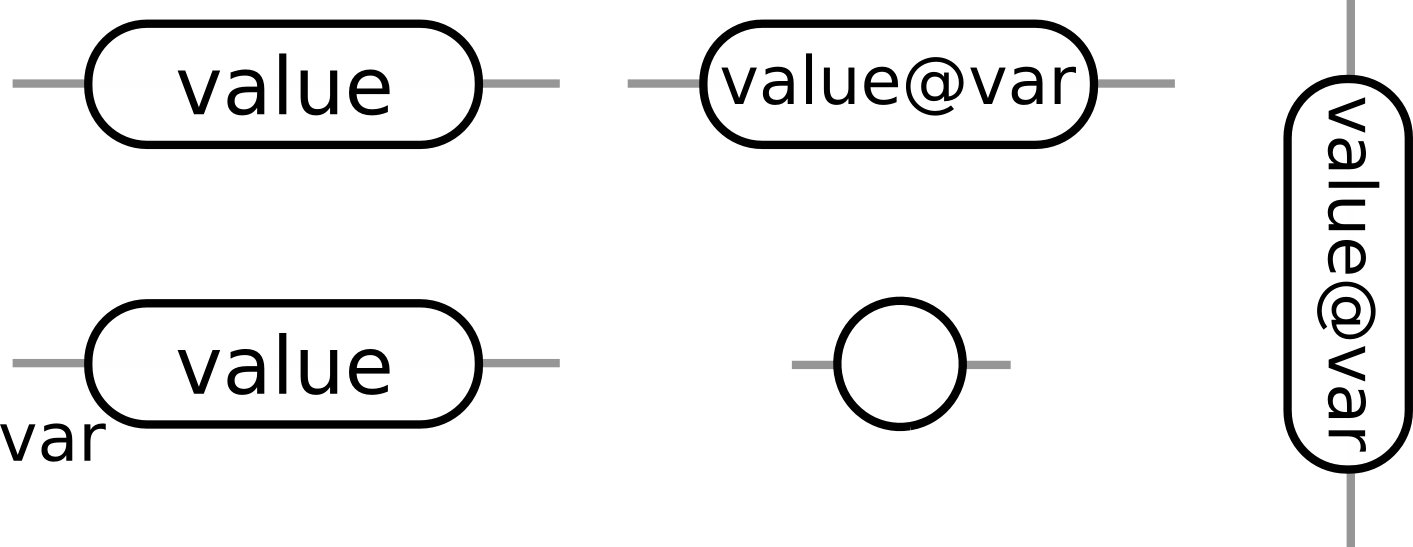
\includegraphics[scale = 0.3, trim = 0 0 0 0.25in]{images/stateVariable}
  \caption{Examples of the \PD glyph for \glyph{state variable}.}
  \label{fig:state-var}
\end{figure}

A \glyph{state variable} does not necessarily have to be Boolean-valued.  For example, an ion channel can possess several conductance states; a receptor can be inactive, active and desensitized; and so on.  As another example, a \glyph{state variable} ``ubiquitin'' could also carry numerical values corresponding to the number of ubiquitin molecules present in the tail.  However, in all cases, a \glyph{state variable} on an EPN can only take \emph{one} defined value.  Further, an EPN's \glyph{state variable} should always be displayed and always set to a value.  An ``empty'' \glyph{state variable} is a \glyph{state variable} that is set to the value ``unset'', it is not a \glyph{state variable} with no value. Note that the value ``unset'' is \emph{not} synonymous to ``any value'' or ``unknown value''.

The label of a \glyph{state variable} should, if possible, be displayed within the ellipse.  In the top half of \fig{wrong-state-var}, we show some examples of pathological cases that lead to confusion in the association between variable labels and values.  Compare the discouraged examples with the recommended version in the bottom half of the figure.

\begin{figure}[H]
  \centering
  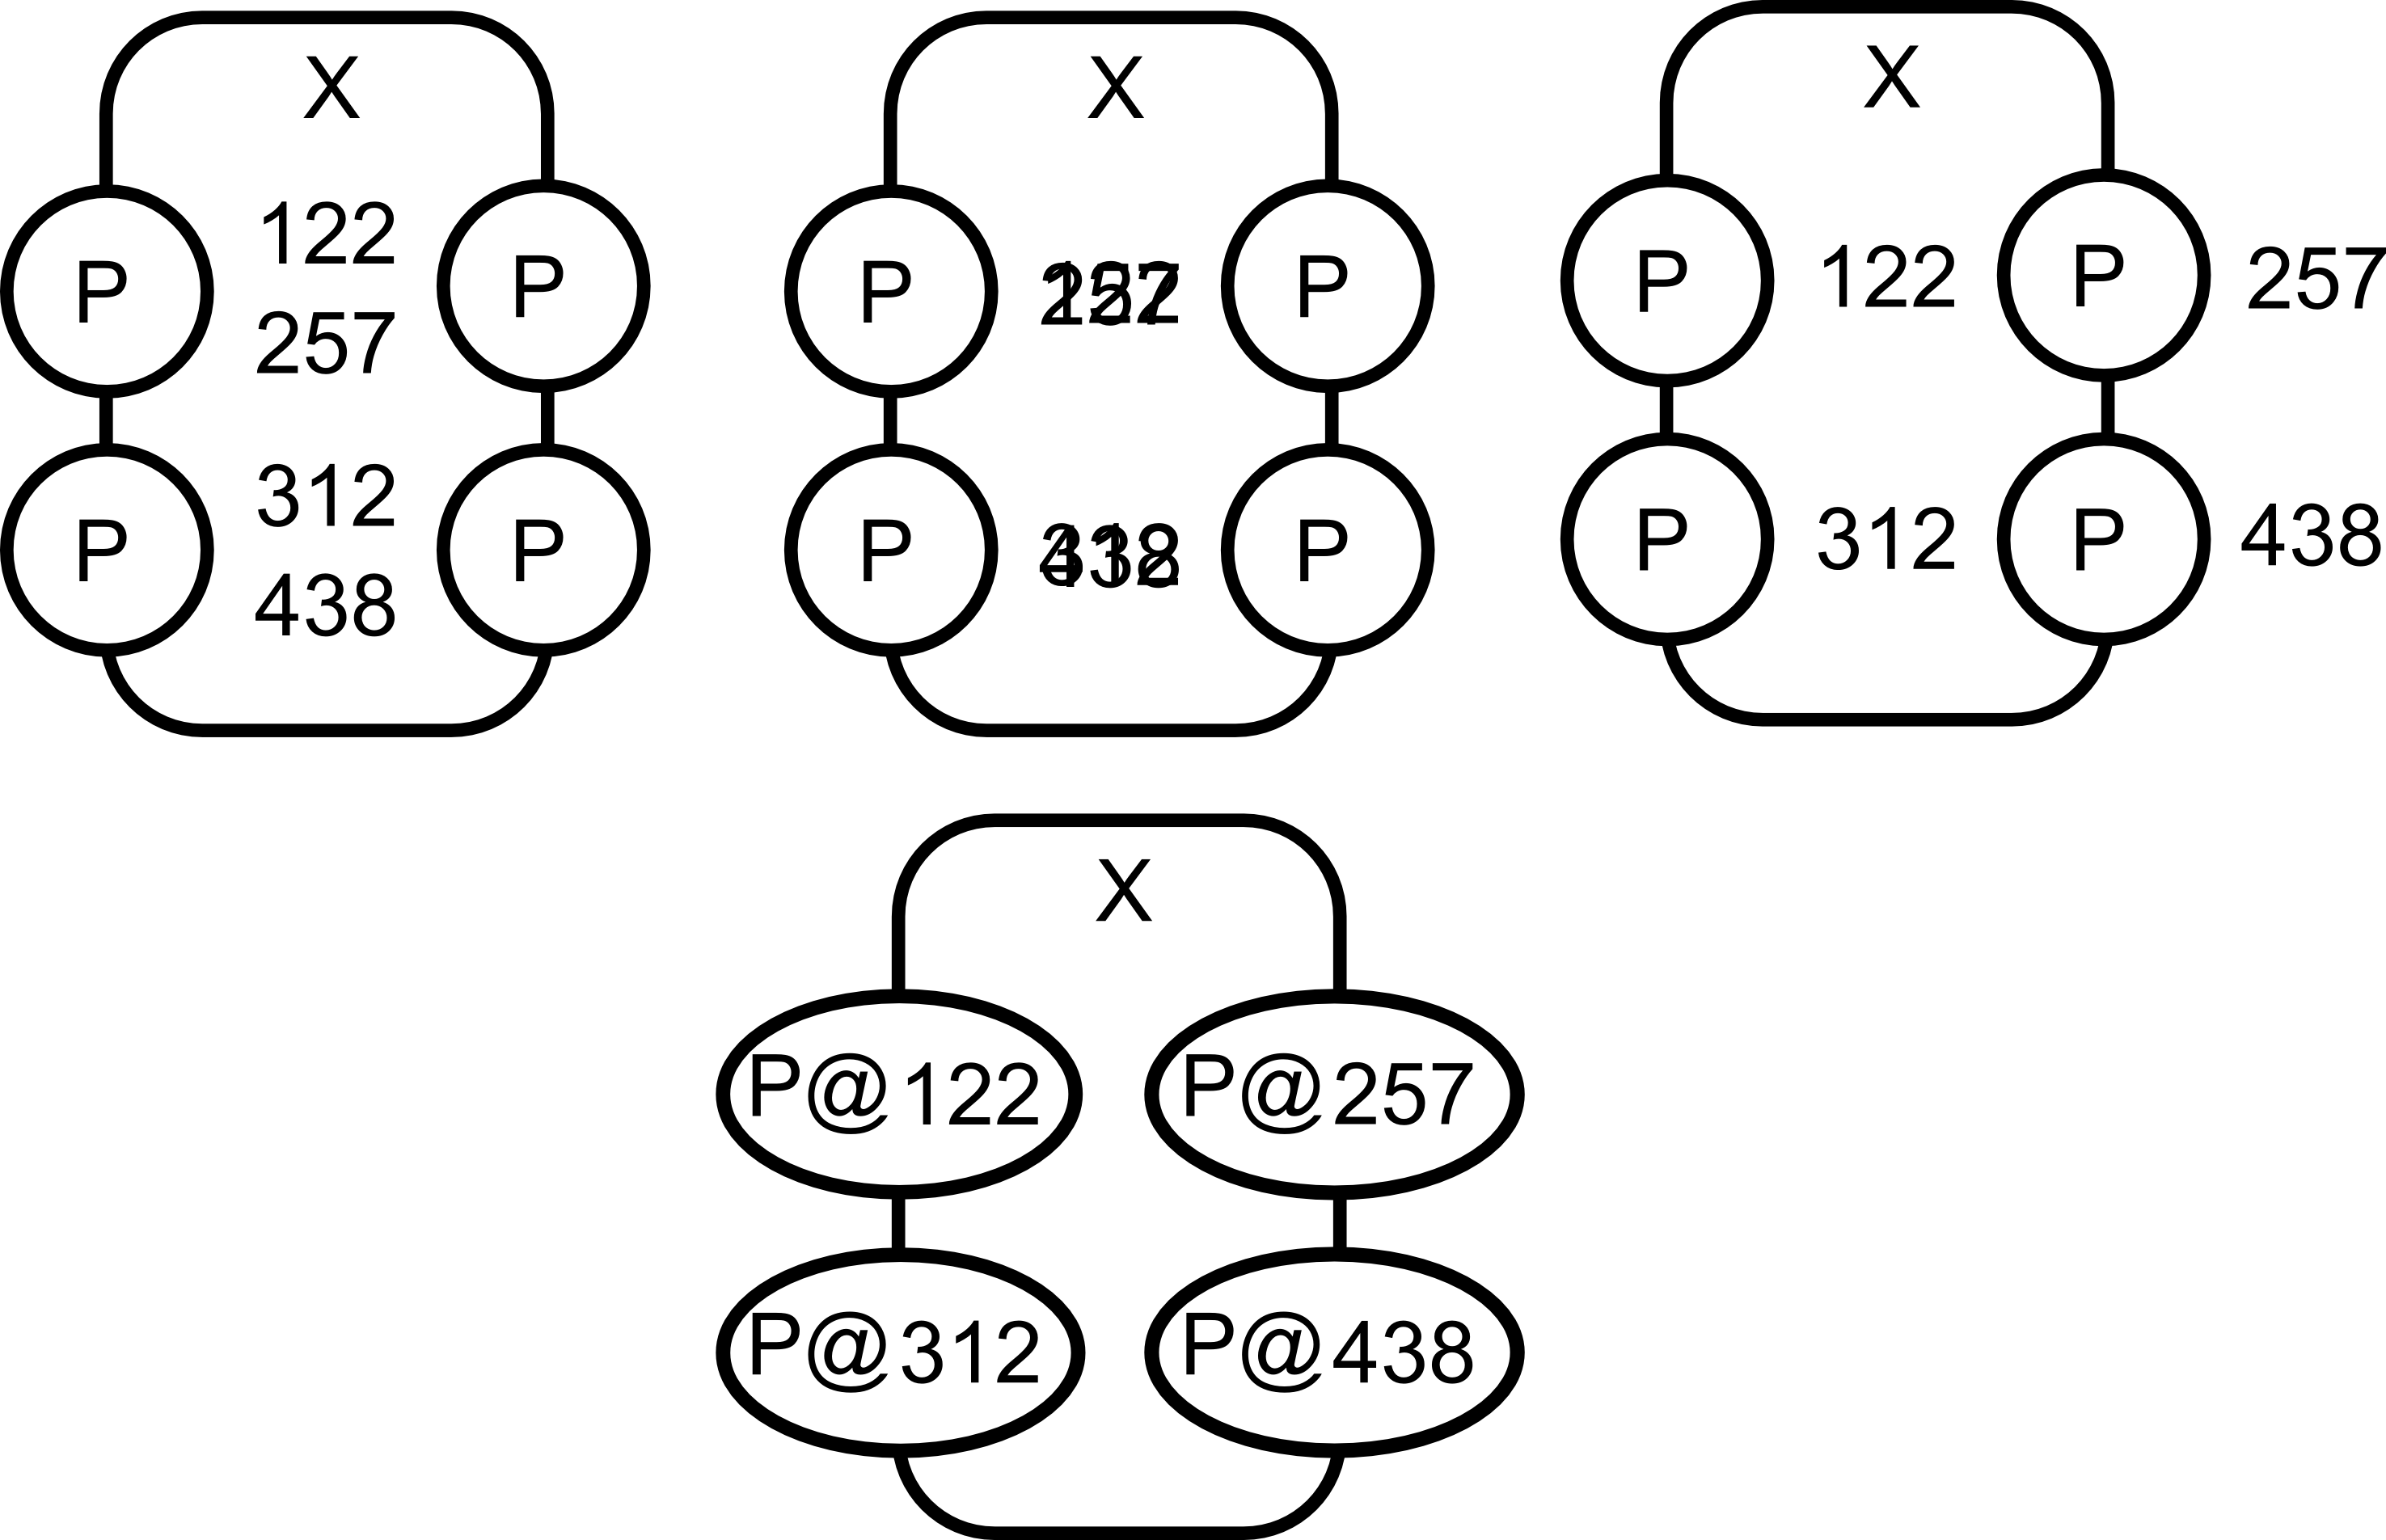
\includegraphics[scale = 0.3, trim = 0 0.5in 0 0.75in]{examples/wrongStateVariables}
  \caption{(Upper part) Examples of incorrect \glyph{state variables}.  (Lower part)
    Correct version.}
  \label{fig:wrong-state-var}
\end{figure}




% The following is for [X]Emacs users.  Please leave in place.
% Local Variables:
% TeX-master: "../sbgn_PD-level1"
% End:

